\begin{block}{Scelta}
    Analizzare \b{tre livelli} crescenti di \b{dettaglio} piuttosto che creare un unico modello onnicomprensivo di pedone.
\end{block}

\begin{block}{Obiettivo}
    Determinare la \b{rilevanza} delle \b{caratteristiche} valutate \b{ripetendo} la stessa \b{simulazione} con \b{diverse tipologie} di agente.
\end{block}

\hfil\hfil
\includegraphics[width=3cm]{images/homogeneous-pedestrian.png}
\hfil\hfil
\includegraphics[width=3cm]{images/heterogeneous-pedestrian.png}
\hfil\hfil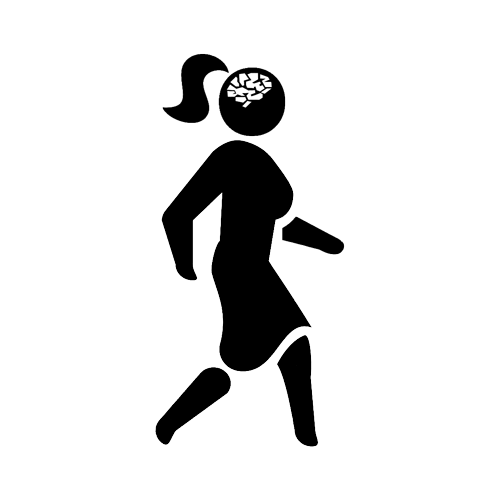
\includegraphics[width=3cm]{images/cognitive-pedestrian.png}\newline
\null
\hfil\hfil\makebox[3cm]{Pedone omogeneo}
\hfil\hfil\makebox[3cm]{Pedone eterogeneo}
\hfil\hfil\makebox[3cm]{Pedone cognitivo}